\section{Introduction}

\begin{figure*}
    \centering
    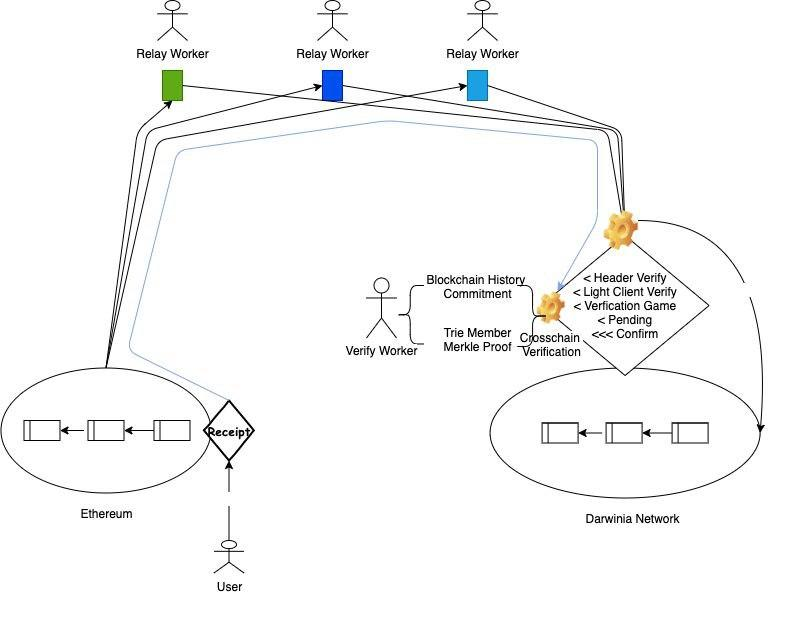
\includegraphics[scale=0.5]{pic/overview.jpg}
    \caption{Overview}
    \label{fig:my_label}
\end{figure*}


There are many efforts on building decentralized bridge between different public chains for supporting swapping, transfer, and more general verification.

Various technologies have been innovated to trying achieve these goals. Hash Time-Locked Contracts(aka. HTLC) are invented to support atomic swap assets in two different public chains, but cannot support asset transfer and verification. To support transfer and verification, several bridges solutions are introduced, including semi-decentralized custodian model and on-chain light client(aka. chain relay) solution.

Chain relay is a light client running on chain with verified headers relayed from another chain's full nodes. Cross-chain verification transactions must be atomic and unstoppable, we need chain relay to confirm the final state of another chain before using it for cross-chain verification. Chain relay is to build and maintain such an on-chain light client with the help of off-chain relayers and on-chan light client verification.

The earliest on-chain light client we know is BTCRelay \cite{btcrelay} built by Consensys, later, Kyber Network also use on-chain light client technologies to build a bi-direction bridge between Ethereum and EOS, which is called WaterLoo \cite{Waterloo}.

This classic chain relay solutions have challenges of economic infeasible due to it is linear relay which means the maintain cost of the relay is growing linear with the block height.

Here we propose a new solution which can resolve this challenges by eliminate the need of relaying each block header from target chain, and achieve a sublinear relay, we call it Darwinia Chain Relay.

To verify events on target chain, the relay need commitment such as merkle roots of events which are commonly recorded in each block header. In darwinia relay, eliminating the need of relaying each block header will result in lacking of these merkle roots, thus we introduce merkle mountain range(MMR)\cite{MMR} as a new commitment representing the header's previous blockchain history. Besides, because the relayed block headers are not continuous chained, this will make light client unable to validate header, darwinia relay resolve header and MMR validation by introducing optimistic verification game\cite{verfG} as sub protocol in relay.

By eliminating the need of relaying each block, darwinia relay can achieve sublinear performance, comparing verifiable blocks on target chain to the fee cost to maintain the relay.

\subsection*{Our contribution}

\begin{itemize}
  \item Through the introduction of an economic incentive mechanism, verification users collect fees from the Relay chain, and incentives are provided to honest block header submitters. For fraudulent block header submissions to Relayer, pledge guarantees are based on Slash-like penalties.
  \item By introducing the Optimistic Verification Game method, the problem of not including MMR in the blockchain head can be solved, and most blockchain protocols can be supported.
  \item Optimistic Verification Game can also solve the problem of malicious attacks under rational economic market games, so it can replace the complex probability-based abstract proof design and heuristic non-interactive design in FlyClient \cite{flyclient}.
  \item Retain the design of MMR and variable difficulty MMR check-in FlyClient design, and realize sub-linear Relay under the premise that the block header is correct
\end{itemize}

The rest of the paper is organized as follows. Section II provides an overview of our entire system. Section III introduces under what circumstances our system is running, and also introduces the definition of some technical indicators of our system. Then, we introduced each component of our system  in section IV with technical details. In the end, we introduced the practical application prospects of this paper.

